\chapter{Implementación}

	\section{¿Qué es una FPAA?}
	Una FPAA  por sus siglas en inglés (Field Programmable Analog Arrays) es un dispositivo analógico equivalente a las FPGA (Field Programmable Garte Arrays). A diferencia de las FPGA que contienen una gran cantidad de módulos y conexiones que permiten configuraciones arbitrarias de lógica combinacional y secuencial, los FPAA generalmente contienen una pequeña cantidad de CABs (Configurable Analog Blocks). Los FPAA dirigidos al diseño analógico estándar generalmente presentan un CAB que contiene un amplificador operacional, un arreglo de capacitores programables, y ya sea un arreglo de resistencias programables para circuitos en tiempo continuo o switches configurables para circuitos de capacitores conmutados.
	Se trabajó con la tarjeta Anadigm QuadApex Develovment Boarsd v2.0 de la empresa Anadigm, la cual contiene 4 FPAAs AN231E04 que pueden conectarse en cadena y es programada mediante el software AnadigmDesigner2 (AD2). El diagrama esquemático de la tarjeta se puede ver en la Figura \ref{fig:esquematico_fpaa} del apéndice.
	
	\section{Características de la tarjeta y requerimientos}
	
	\subsection{Alimentación de la tarjeta}
	Para el correcto funcionamiento de la placa esta debe ser alimentada con una fuente de voltaje regulada a 5V de al menos 500mA conectada a la clema de dos terminales. Hay un LED de color verde que indica que la placa se ha encendido correctamente, la placa esta protegida contra la conexión de una fuente de voltaje con la polarización incorrecta.
	
	\subsection{Instalación de drivers}

No conecte la placa QuadApex v2.0 a la PC vía cable USB,  ni tampoco inicie AD2 ahora, el driver debe instalarse primero. Se asume que AD2 ya ha sido instalado y registrado en su computadora, de lo contrario entre al link que aparece a continuación.

Para instalar AD2 basta con acceder al siguiente link y seguir los pasos que muestra la pagina:

	\begin{center}
		\url{https://www.anadigm.com/sup_downloadcenter.asp?tab=ad2}
	\end{center}

es recomendable guardar los datos de registro en un lugar seguro, al iniciar el programa por primera vez es necesario ingresar el \textbf{License ID} y la \textbf{License key} estos estarán en el correo que le proporcionó a Anadigm. 

El driver \textbf{CP210x\_{}Drivers.exe} está incluido en el AD2 CD o se puede encontrar en la página de Silicon Labs. Siga los siguientes pasos si es la primera vez que instala este driver, de lo contrario desinstale las versiones anteriores antes de continuar:

\begin{enumerate}
	\item Ejecute como administrador el ejecutable  CP210x\_{}Drivers.exe. El destino por defecto del ejecutable es ‘‘C:\textbackslash{}Silabs\textbackslash{}Mcu\textbackslash{}CP210x’’.
	\item Para completar la instalación conecte la QuadApex v2.0 y enciéndala.
	\item Acceda al administrador de dispositivos y en \textbf{Puertos (COM y LPT)} asegúrese que el driver este bien configurado, si no aparece un signo de admiración y se le asigno un puerto COM  la instalación fue exitosa, de lo contrario dar clic derecho sobre el dispositivo y seleccionar \textbf{Actualizar controlador}, después buscar el  driver en la ruta del paso 1.
\end{enumerate}

El driver en este punto ya esta instalado. La instalación del driver y la asignación del puerto es necesaria solo una vez. Si se conecta subsecuentemente a otro puerto de USB de la PC puede ser necesario repetir el paso 3.

	\subsection{DIP Switches}
	
	El usuario puede hacer sus propias conexiones en la placa con cables, pero hay un conjunto de DIP switches que permiten una fácil conexión de ciertas rutas entre los FPAA vecinos y entre los FPAA y los \textbf{input/output buffers}. Estos interruptores están abiertos por defecto, lo que significa que todos están hacia la izquierda. El usuario puede cerrar los interruptores empujándolos hacia la derecha. En la Tabla \ref{tab:switches} se muestra un resumen de los switches. Los DIP switches son pequeños y del tipo deslizantes, por lo que se recomienda una herramienta afilada como un destornillador delgado para abrir ycerrar los switches.

	\begin{table}[!ht]
		\centering
		\begin{tabular}{|l|l|l|}
			\hline
			\textbf{Función} &  \textbf{Tipo} & \textbf{Labels}\\
			\hline
			Conectar filtros Rauch a FPAA i/ps 					& 4way 		& S8,9,10,11,15,16,17,18		\\
			\hline
			Conectar entre FPAAs 						& 4way 	& S2,3,4,5,6,7	\\
			\hline
			Conectar FPAA o/ps a buffers 						& 2way 		& S12,13,14,19		\\
			\hline
		\end{tabular}
		\caption{DIP Switches}
		\label{tab:switches}
	\end{table}



	
	\subsection{Filtros Rauch y buffers de salida}
	
	La tarjeta cuenta con 2 buffers de entrada llamados filtros Rauch listos para usar, \textbf{Rauch\_\#1\_I01} y \textbf{Rauch\_\#2\_I01}, estos son filtros multipropósito no obstante su principal función es convertir una señal single-ended a una diferencial en la FPAA, internamente la FPAA trabaja únicamente con señales diferenciales y debido a esto el uso de estos filtros es imprescindibles para introducir señales externas, por ejemplo de generadores de funciones u otros circuitos. Si se usa una señal single-ended, es necesario conectar IN- a GND y conectar la señal a IN+.
	Para activar el filtro es necesario hacerlo desde el software AD2 haciendo doble clic en la IO cell apropiada (IOCell1-4), seleccionar Input y después Amplifier.
	
	Rauch\_\#1\_I01 está conectado a I/O1 de la FPAA \#1 y esta configurado con una frecuencia de corte muy alta y ganancia unitaria ($F_{o} = 490$KHz)
	
	Para habilitar el amplificador en AD2, haga doble clic en la IO cell apropiada (IOCell1-4), seleccione el radio button marcado Input, después seleccione el radio button marcado Amplifier
	\section{AnadigmDesigner2}
	
	AD2 trabaja con módulos llamados CAMs (Configurable Analog Modules), estos aportan flexibilidad y sencillez en el proceso diseño debido a que son bloques que hacen desde funciones sencillas como inversores o comparadores hasta diseños completos como filtros y multiplicadores, los CAMs se pueden interconectarse fácilmente unos con otros y únicamente necesitan pequeñas configuraciones para su correcto funcionamiento. Los CAMs más utilizados en el diseño de osciladores caóticos son los mostrados en la Tabla \ref{tab:CAMs_AD2}.
	

\begin{table}[!ht]
  \centering
  \caption{CAMs básicos de AD2}
  \label{tab:CAMs_AD2}
  \begin{tabular}{>{\centering\arraybackslash}m{3cm} >{\centering\arraybackslash}m{5cm} >{\centering\arraybackslash}m{5cm}}
    \hline
    \textbf{Nombre} & \textbf{Función de transferencia} & \textbf{Descripción}\\ 
    \hline
    {\scriptsize \textbf{GainInv}}
    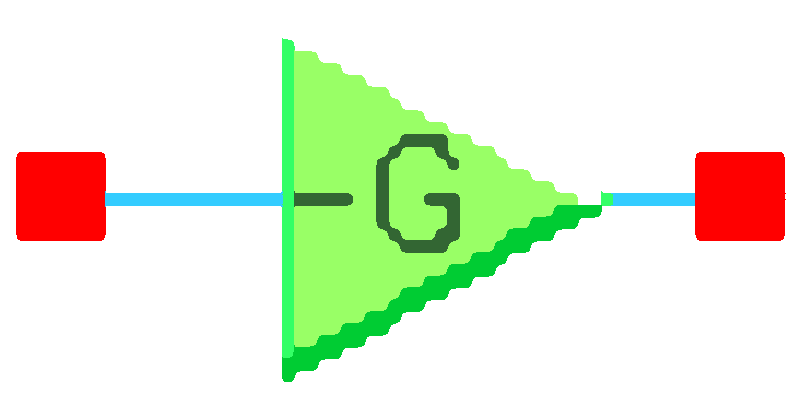
\includegraphics[width=2.2cm]{T7_Inversor.eps}
    &
      $\frac{V_{\mathrm{out}} (s)}{V_{\mathrm{in}}(s)} = - G$
    & 
      \begin{itemize}[leftmargin=0cm,noitemsep]
      \begin{scriptsize}
		\item[] Ganancia inversora.
		\item[] Gain: 0.01 - 100.0 V/V
      \end{scriptsize}
      \end{itemize}
    \\ %-------------------------------------------------------
    {\scriptsize \textbf{Integrator}}
    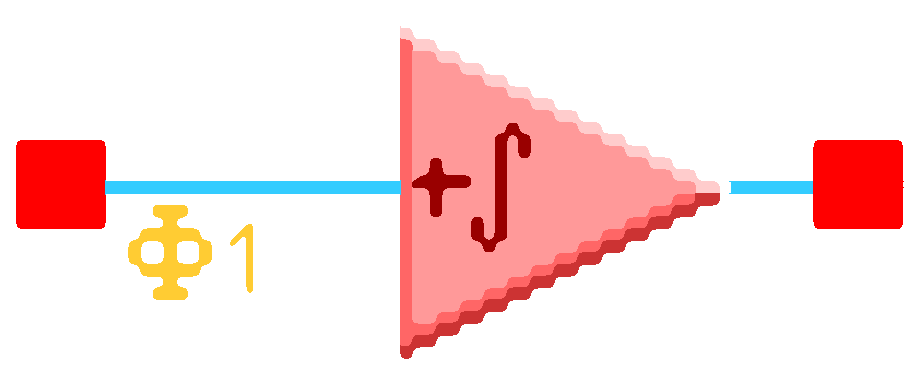
\includegraphics[width=2.5cm]{T1_Integrador.eps}
    &
      $ \frac{V_{\mathrm{out}} (s)}{V_{\mathrm{in}}(s)} = \frac{\pm K}{s}$
    & 
      \begin{itemize}[leftmargin=0cm,noitemsep]
      \begin{scriptsize}
		\item[] Integrador con una constante de integración programable. La salida puede ser inversora o no inversora.
      \end{scriptsize}
      \end{itemize}
    \\ %-------------------------------------------------------
    {\scriptsize \textbf{Voltage}} \linebreak
    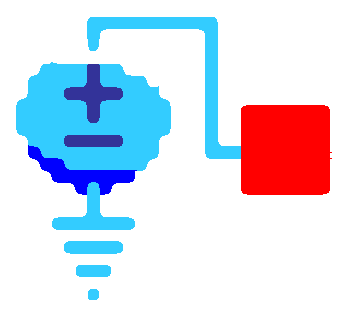
\includegraphics[width=1cm]{T6_DC_voltage.eps}
    &
      $V_{\mathrm{out}} = \pm 2$
    & 
      \begin{itemize}[leftmargin=0cm,noitemsep]
      \begin{scriptsize}
		\item[] Referencia de voltaje de $\pm$ 2 V.
      \end{scriptsize}
      \end{itemize}
    \\ %-------------------------------------------------------
    {\scriptsize \textbf{TransferFunction}} \linebreak
    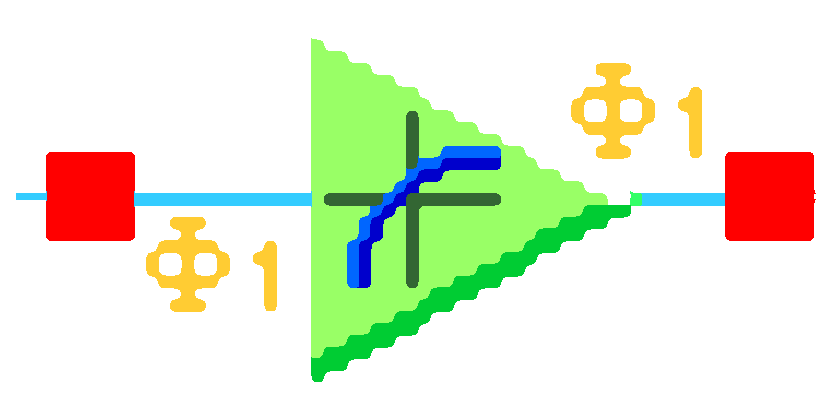
\includegraphics[width=2.5cm]{T3_Transferfunction.eps}
    &
    & 
      \begin{itemize}[leftmargin=0cm,noitemsep]
      \begin{scriptsize}
		\item[] \textbf{Lookup Table}: función de transferencia especificada por el usuario de 256 de pasos de cuantificación.  
      \end{scriptsize}
      \end{itemize}
    \\ %-------------------------------------------------------
    {\scriptsize \textbf{Multiplier}} \linebreak
    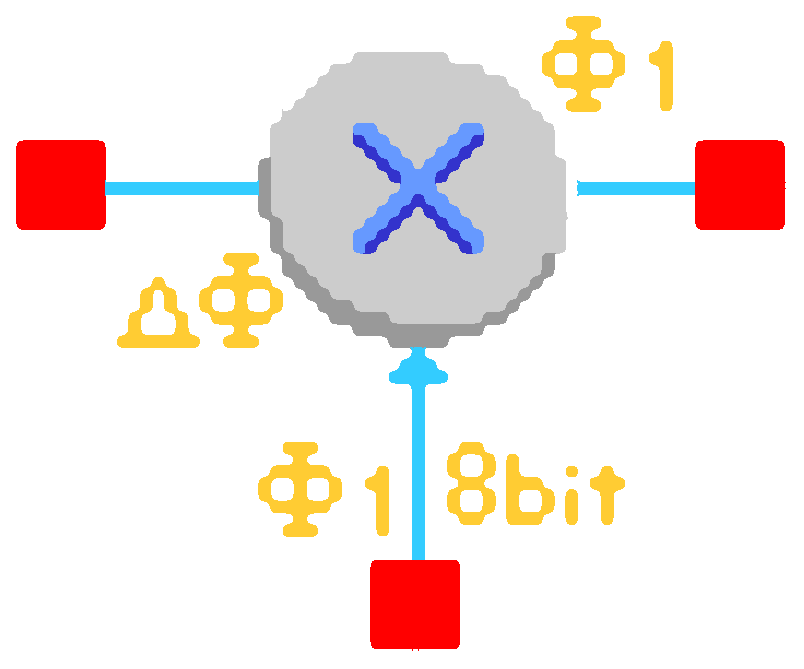
\includegraphics[width=2.5cm]{T2_Multiplicador.eps}
    &
      $V_{\mathrm{out}} = M \cdot V_{x} \cdot V_{y}$
    & 
      \begin{itemize}[leftmargin=0cm,noitemsep]
      \begin{scriptsize}
		\item[] $V_{x}$ es la entrada de voltaje izquierda.
		\item[] $V_{y}$ es la entrada de voltaje inferior cuantificado de 8 bits.
		\vspace{-0.15cm}
		\item[] $M$ factor de multiplicación.
      \end{scriptsize}
      \end{itemize}
    \\ %-------------------------------------------------------
    {\scriptsize \textbf{SumDiff}} \linebreak
    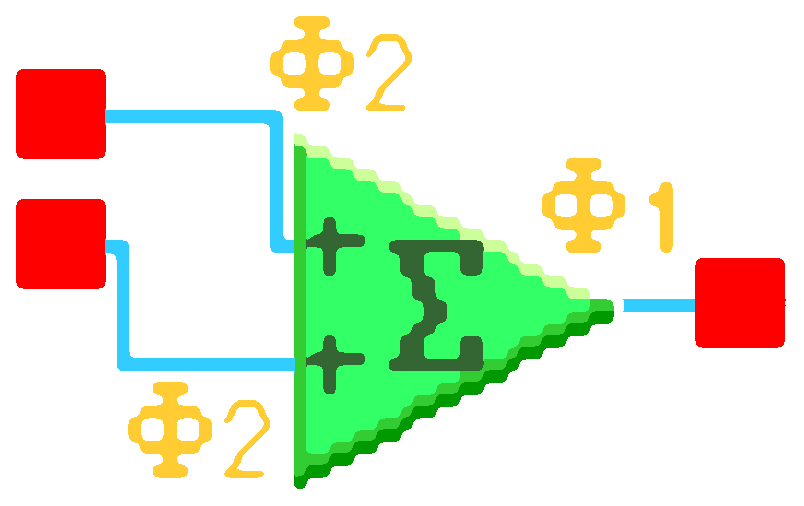
\includegraphics[width=2.5cm]{T8_Sumador.eps}
    &
      \begin{footnotesize}
      	$V_{\mathrm{out}} = \pm G_{1} V_{\mathrm{in1}} \pm G_{2} V_{\mathrm{in2}} \pm G_{3} V_{\mathrm{in3}} \pm G_{4} V_{\mathrm{in4}}$
      \end{footnotesize}
    & 
      \begin{itemize}[leftmargin=0cm,noitemsep]
      \begin{scriptsize}
		\item[] Las entradas pueden ser inversoras o no inversoras.
		\item[]	Cada entrada tiene una ganancia programable.
		\vspace{-0.15cm}
		\item[] Configurable desde 2 hasta 4 entradas. 
      \end{scriptsize}
      \end{itemize}
    \\ %-------------------------------------------------------
    {\scriptsize \textbf{FilterBilinear}} \linebreak
    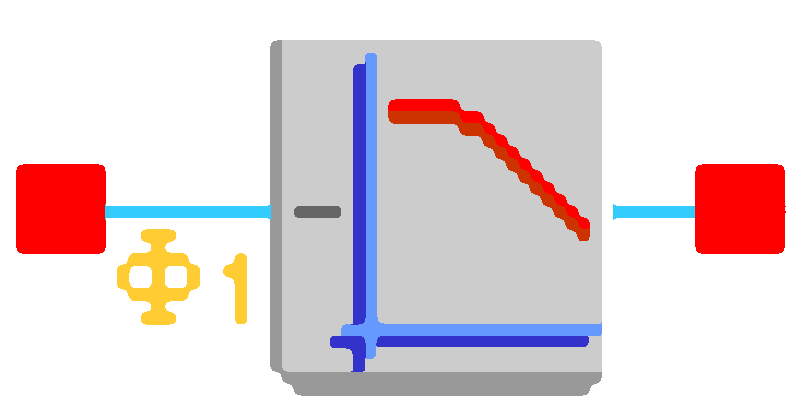
\includegraphics[width=2.5cm]{T9_FilterBilinear.eps}
    &
      \begin{scriptsize}
		 \textbf{Low Pass Bilinear Filter} \linebreak
      	 $\frac{V_{\mathrm{out}}(s)}{V_{\mathrm{in}}(s)} = \pm \frac{2 \pi f_{0} G}{s + 2 \pi f_{0}}$ \linebreak
      	 \textbf{High Pass Bilinear Filter} \linebreak
      	 $\frac{V_{\mathrm{out}}(s)}{V_{\mathrm{in}}(s)} = - \frac{Gs}{s + 2 \pi f_{0}}$ \linebreak
      	 $\vdots$
      \end{scriptsize}
    & 
      \begin{itemize}[leftmargin=0cm,noitemsep]
      \begin{scriptsize}
		\item[] Puede ser configurado como pasabajas, pasaaltas, pasatodas o general (Polo y cero).
      \end{scriptsize}
      \end{itemize}
    \\ %-------------------------------------------------------
    {\scriptsize \textbf{FilterBiquad}} \linebreak
    \includegraphics[width=2.5cm]{T10_FilterBiquad.eps}
    &
      \begin{scriptsize}
		 \textbf{Low Pass Biquadratic Filter} \linebreak
      	 $\frac{V_{\mathrm{out}}(s)}{V_{\mathrm{in}}(s)} = \frac{\pm 4 \pi^{2} f_{0}^{2} G}{s^{2} + \frac{2 \pi f_{0}}{Q}s + 4 \pi^{2} f_{0}^{2}}$ \linebreak
      	 \textbf{High Pass Biquadratic Filter} \linebreak
      	 $\frac{V_{\mathrm{out}}(s)}{V_{\mathrm{in}}(s)} = \frac{-G s^{2}}{s^{2} + \frac{2 \pi f_{0}}{Q} s + 4 \pi^{2} f_{0}^{2}}$ \linebreak
      	 $\vdots$
      \end{scriptsize}
    & 
      \begin{itemize}[leftmargin=0cm,noitemsep]
      \begin{scriptsize}
		\item[] Puede ser configurado como pasabajas, pasaaltas, pasabanda, rechazabanda o general (Polos y ceros).
      \end{scriptsize}
      \end{itemize}
    \\ %-------------------------------------------------------
    \hline
  \end{tabular}
\end{table}

	Las configuraciones de los CAMs dependen de las frecuencias de reloj que se seleccionen para cada FPAA. Cada FPAA tiene dos fuentes de frecuencias de reloj principales \textbf{Sys1} y \textbf{Sys2}, y cinco frecuencias de reloj de chip, desde \textbf{Clock 0} hasta \textbf{Clock 5} que son subdivisiones de cualquiera de las fuentes de reloj principales. Seleccionar y configurar correctamente los relojes es importante ya que el rango de operación de los CAMs depende de esto. 

	\section{Implementación con aproximación de primer orden}
	
	Para realizar la implementación física de la aproximación de primer orden del integrador fraccionario se utilizó el CAM \textbf{FilterBilinear} en su modo \textbf{Pole and Zero}, esto debido a su flexibilidad y semejanza con la función de transferencia de la aproximación de la CFE de primer orden. La función de transferencia del CAM en este modo es la siguiente:
	
	\begin{equation}
		\frac{V_{\mathrm{out}} (s)}{V_{\mathrm{in}}(s)} = -\frac{G_{H} (s + 2 \pi f_{z})}{s + 2 \pi f_{p}}
	\end{equation}
	donde $G_{L}$ esta definida como:
	\begin{equation}
		G_{L} = \frac{f_{z}}{f_{p}} G_{H}
	\end{equation}
	y donde $G_{L}$ es la ganancia en DC, $G_{H}$ es la ganancia de alta frecuencia, $f_{p}$ es la frecuencia del polo y $f_{z}$ es la frecuencia del cero.
	
	La función de transferencia de la aproximación con la CFE de primer orden, como se mencionó anteriormente es la siguiente:
	\begin{equation}
		\genfrac{}{}{0pt}{0}{}{_{(c_{2})}} \frac{1}{s^{\alpha}} \approx \frac{(1 - \alpha)s + (1 + \alpha) }{(1 + \alpha)s + (1 - \alpha)} 
		\label{ec:cfe_primer_orden}
	\end{equation}
	si consideramos la siguiente sustitución:
	
	\begin{equation}
		A = \frac{1 - \alpha}{1 + \alpha}
	\end{equation}
	podemos reescribir la ecuación (\ref{ec:cfe_primer_orden}) de la siguiente manera:
	
	\begin{equation}
		\genfrac{}{}{0pt}{0}{}{_{(c_{2})}} \frac{1}{s^{\alpha}} \approx \frac{A s + 1}{s + A}
		\label{ec:cfe_primer_orden_simp}
	\end{equation}
	aplicando el escalamiento en frecuencia a la ecuación (\ref{ec:cfe_primer_orden_simp}) se convierte en:
	
	\begin{equation}
		\frac{A s + k_{f}}{s + A k_{f}}
		\label{ec:cfe_primer_orden_simp_esc}
	\end{equation}
	